\chapter{Fase 1: requisitos da avaliação}
\label{cap:fase1}

A Fase 1 estabelece o que será avaliado, por quê, para quem e com que profundidade \cite{iso25040,ramos2026processo}. As páginas detalhadas de cada decisão estão na seção ``Fase 1'' da GitPage.

\section{Propósito e partes interessadas}
\label{sec:proposito}

O propósito da avaliação é \textbf{identificar, com evidências mensuráveis, os pontos fracos do SIGAA nas tarefas acadêmicas mais frequentes do estudante de graduação}, para apoiar a priorização de melhorias pela STI/UnB e embasar a ação de melhoria exigida na Fase 4. O ponto de vista é o do estudante, com atenção a perfis vulneráveis: calouros, que desconhecem a terminologia acadêmica; estudantes que acessam o sistema apenas pelo celular; e estudantes com deficiência. Veteranos e formandos servem de contraste: problemas que persistem mesmo com experiência indicam falhas de operabilidade, e o formando exercita as funções mais críticas (histórico, índices e carga horária pendente).

A demanda formal parte da disciplina FGA0315, que define o processo e os critérios de aceitação, e os resultados destinam-se à STI/UnB (operadora local do sistema), ao Decanato de Ensino de Graduação (DEG) e às coordenações de curso, à comunidade estudantil e à UFRN, desenvolvedora do produto. A \autoref{tab:decisoes} relaciona as decisões que a avaliação apoia, quem as toma e o resultado que as embasa.

\begin{table}[htb]
	\caption{Decisões apoiadas pela avaliação}
	\label{tab:decisoes}
	\centering
	\scriptsize
	\begin{tabularx}{\textwidth}{Y L{2.3cm} Y}
		\toprule
		\textbf{Decisão} & \textbf{Quem decide} & \textbf{Resultado que a embasa} \\
		\midrule
		Quais telas e fluxos do portal do discente priorizar em um ciclo de melhoria & STI/UnB & Ranking das tarefas com pior desempenho em Capacidade de Interação e Adequação Funcional \\
		Investir ou não em interface responsiva ou aplicativo móvel & STI/UnB & Flexibilidade cruzada com o perfil de acesso dos estudantes \\
		Quais procedimentos precisam de tutorial ou orientação adicional & DEG e coordenações & Tarefas com maior taxa de erro ou abandono e funções de difícil localização \\
		Se é necessário otimizar páginas específicas (peso, requisições) & STI/UnB & Comportamento temporal e uso de recursos por página \\
		Qual ação de melhoria executar na Fase 4 & Equipe & Problema de maior impacto entre os julgamentos \\
		\bottomrule
	\end{tabularx}
	\fonte{Elaborado pela equipe.}
\end{table}

\section{Produto avaliado}
\label{sec:produto}

O objeto é o \textbf{portal do discente de graduação do SIGAA/UnB}, versão v4.15.10.115 (informada no rodapé do sistema em 16/10/2026), acessado pela interface web em produção (\autoref{fig:portal}) \cite{sigaa}. Trata-se de um sistema de informação web, transacional e institucional, construído em JavaServer Faces e acessado pela Autenticação Integrada compartilhada com os demais sistemas SIG. Pela classificação da IEEE 1062 apresentada na disciplina, é um produto MOTS (\textit{Modified Off-The-Shelf}): um produto-padrão da UFRN implantado com configurações próprias por cada instituição \cite{ramos2026processo}. Para a equipe, é um produto de código fechado, o que restringe a avaliação ao comportamento observável: é possível medir tempo de carregamento no navegador, conclusão e esforço nas tarefas, comportamento em navegadores e telas e conformidade com critérios de acessibilidade, mas não o processamento no servidor, o comportamento sob carga ou a qualidade do código.

\begin{figure}[htb]
	\centering
	\caption{Página inicial do portal do discente do SIGAA/UnB}
	\label{fig:portal}
	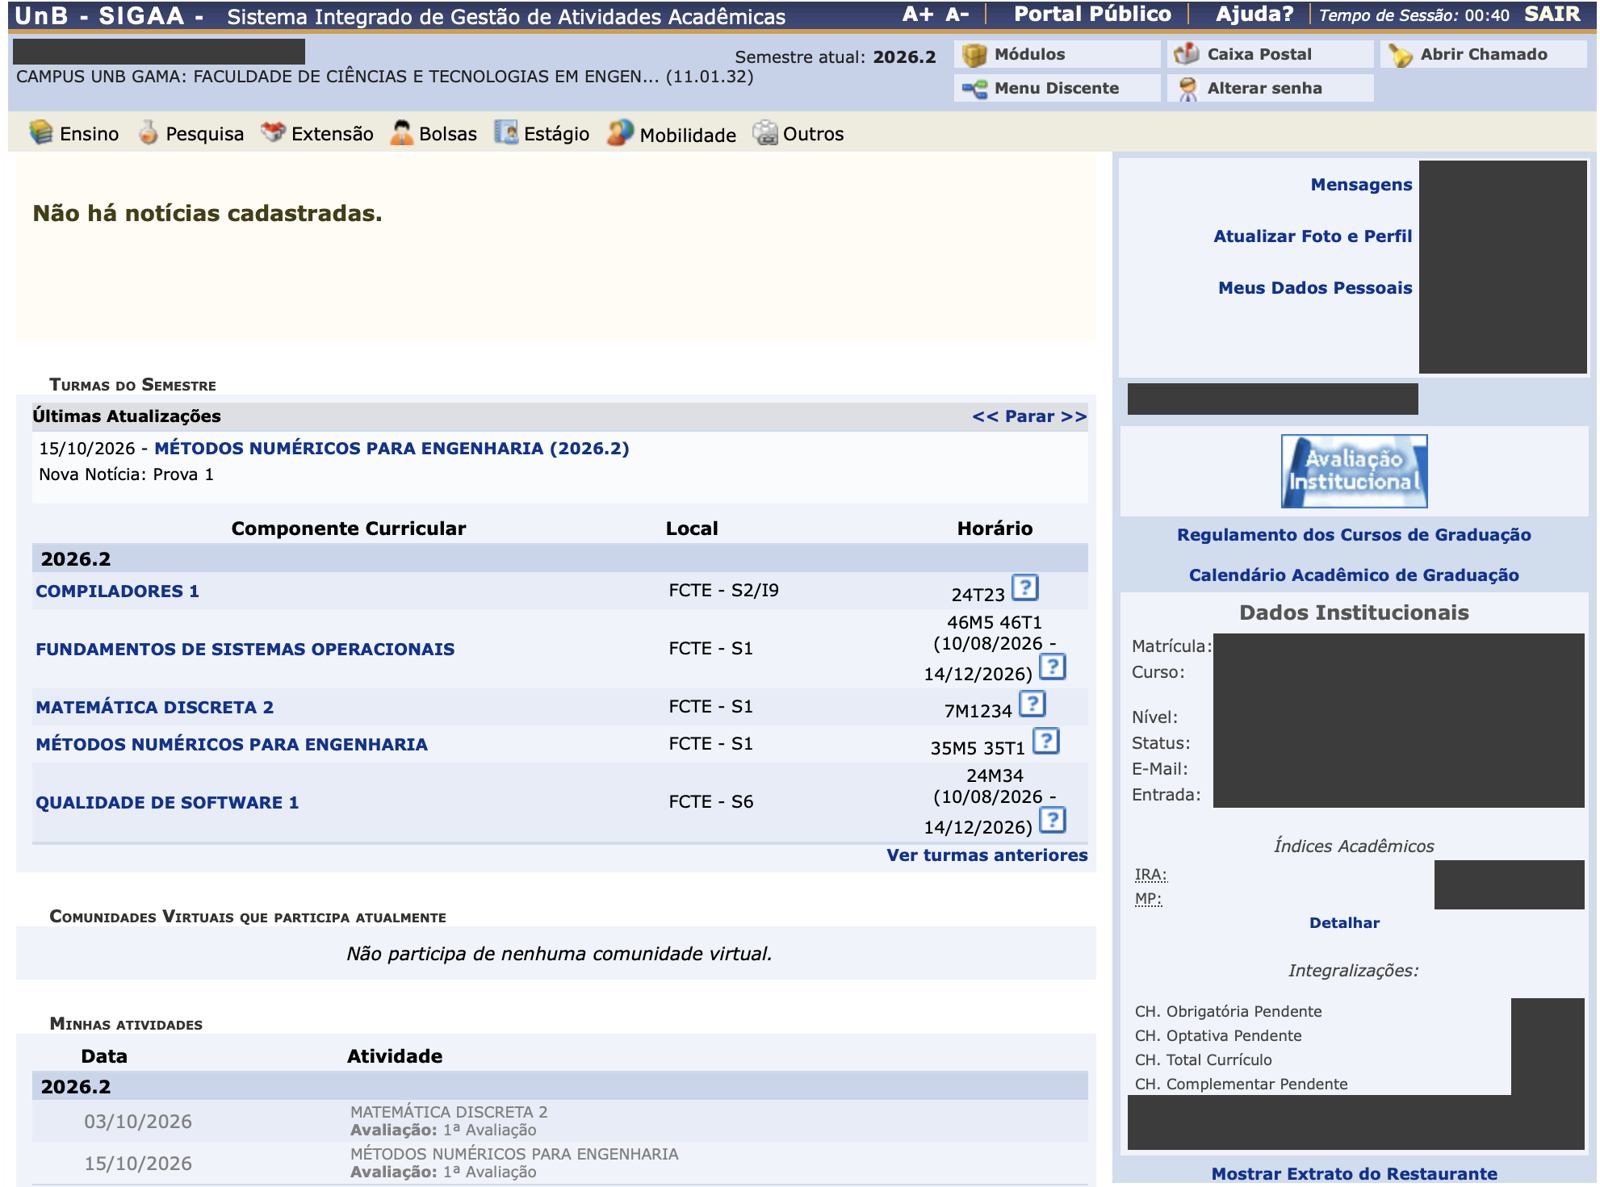
\includegraphics[width=0.82\textwidth]{figuras/sigaa-portal-discente.png}
	\fonte{Captura da equipe em 16/10/2026, com dados pessoais ocultados.}
\end{figure}

A inspeção inicial produziu oito observações preliminares (OP), que não são resultados, mas indícios que orientaram a seleção das características e serão verificados na Fase 4 (\autoref{tab:op}).

\begin{table}[htb]
	\caption{Observações preliminares da interface}
	\label{tab:op}
	\centering
	\scriptsize
	\begin{tabularx}{\textwidth}{C{0.9cm} Y L{4.4cm}}
		\toprule
		\textbf{ID} & \textbf{Observação} & \textbf{Característica relacionada} \\
		\midrule
		OP-01 & Horários das turmas em notação codificada (``24M34''), interpretável apenas com uma legenda & Capacidade de Interação (autodescritividade) \\
		OP-02 & Menus suspensos abertos pela passagem do ponteiro, sem equivalente evidente para toque & Flexibilidade; Capacidade de Interação \\
		OP-03 & Layout de largura fixa, sem adaptação ao tamanho da janela & Flexibilidade (adaptabilidade) \\
		OP-04 & Menu Ensino com cerca de 20 itens em um único nível, misturando consultas, documentos e matrícula & Capacidade de Interação (reconhecimento de adequação) \\
		OP-05 & Duas estruturas de navegação: menus horizontais no portal e menu lateral na Turma Virtual & Capacidade de Interação (operabilidade) \\
		OP-06 & Sessão com expiração por inatividade e contador no cabeçalho & Capacidade de Interação (proteção contra erros) \\
		OP-07 & Ferramentas comunitárias para planejar o fluxo de disciplinas, função ausente ou insuficiente no sistema & Adequação Funcional (completude) \\
		OP-08 & Recurso de aumento e redução de fonte (A+/A-) no cabeçalho & Capacidade de Interação (inclusividade), ponto positivo \\
		\bottomrule
	\end{tabularx}
	\fonte{Elaborado pela equipe.}
\end{table}

\section{Modelo de qualidade e priorização das características}
\label{sec:priorizacao}

O modelo de referência é o da ISO/IEC 25010:2023 (\autoref{tab:iso25010}), adaptado ao contexto por três filtros: relevância para as partes interessadas, mensurabilidade em avaliação caixa-preta e viabilidade ética, pois nenhum teste pode alterar dados reais, sobrecarregar o ambiente de produção ou violar termos de uso.

Para escolher de três a quatro características, cada membro atribuiu notas de 1 a 5 de \textbf{impacto} ($I$), a consequência de uma deficiência para as partes interessadas, e de \textbf{risco} ($R$), a probabilidade de deficiência estimada pelas observações preliminares, pela idade da tecnologia e por relatos dos estudantes. As notas foram consolidadas em reunião, e a prioridade é $P = I \times R$. Foram selecionadas as características viáveis com $P \geq 15$, limitadas a quatro (\autoref{tab:matriz}).

\begin{table}[htb]
	\caption{Matriz Impacto $\times$ Risco das características da ISO/IEC 25010:2023}
	\label{tab:matriz}
	\centering
	\scriptsize
	\begin{tabularx}{\textwidth}{L{3.4cm} C{0.5cm} C{0.5cm} C{0.9cm} C{1.4cm} Y}
		\toprule
		\textbf{Característica} & \textbf{$I$} & \textbf{$R$} & \textbf{$P$} & \textbf{Viável} & \textbf{Decisão e justificativa} \\
		\midrule
		Capacidade de Interação & 5 & 5 & \textbf{25} & Sim & Selecionada (prioridade 1): seis das oito OP; afeta todos os perfis \\
		Adequação Funcional & 5 & 4 & \textbf{20} & Sim & Selecionada (2): dado errado ou função ausente compromete decisões acadêmicas (OP-07) \\
		Eficiência de Desempenho & 4 & 4 & \textbf{16} & Parcial & Selecionada (3): lentidão atrasa todas as tarefas e pesa mais em rede móvel \\
		Flexibilidade & 4 & 4 & \textbf{16} & Parcial & Selecionada (4): layout fixo e menus por ponteiro (OP-02, OP-03) \\
		Confiabilidade & 4 & 3 & 12 & Parcial & Preterida: falhas concentram-se na matrícula, fora da janela de coleta \\
		Segurança & 5 & 2 & 10 & Não & Preterida: exigiria testes de invasão não autorizados \\
		Manutenibilidade & 3 & 3 & 9 & Não & Preterida: sem acesso ao código-fonte \\
		Compatibilidade & 2 & 2 & 4 & Parcial & Preterida: integração não observável pelo estudante \\
		Segurança Operacional & 1 & 1 & 1 & -- & Preterida: o sistema não controla processos físicos \\
		\bottomrule
	\end{tabularx}
	\fonte{Elaborado pela equipe.}
\end{table}

Dentro das características selecionadas, foram mantidas apenas as subcaracterísticas mensuráveis no contexto: em Capacidade de Interação, engajamento e assistência ao usuário foram removidas por serem subjetivas demais para o prazo e por dependerem de canais fora da interface; em Eficiência de Desempenho, a capacidade foi removida por exigir testes de carga; em Flexibilidade, apenas a adaptabilidade foi mantida, pois instalabilidade e substituibilidade não se aplicam a um sistema web e a escalabilidade exige acesso ao servidor. O principal custo dessa seleção é que a avaliação descreve a qualidade do sistema em uso pelo estudante, e não a robustez interna da implementação. Para não perder informação, falhas observadas durante as tarefas serão registradas como não conformidades de Adequação Funcional.

\section{Escopo, tarefas e rigor}
\label{sec:escopo}

A avaliação é organizada em torno de seis tarefas representativas, escolhidas por frequência de uso, criticidade e disponibilidade durante a coleta (\autoref{tab:tarefas}). Todas são executadas em computador e celular, nos navegadores Chrome, Firefox, Safari e Edge, em telas de cerca de 360~px, 768~px e 1280~px, e em rede comum e móvel simulada.

\begin{table}[htb]
	\caption{Tarefas representativas que compõem o escopo}
	\label{tab:tarefas}
	\centering
	\scriptsize
	\begin{tabularx}{\textwidth}{C{0.6cm} Y L{4.6cm}}
		\toprule
		\textbf{ID} & \textbf{Tarefa} & \textbf{Caminho principal no sistema} \\
		\midrule
		T1 & Consultar as notas de uma disciplina do semestre & Ensino > Consultar Minhas Notas \\
		T2 & Identificar dia, horário e local de uma turma & Página inicial > Turmas do semestre \\
		T3 & Emitir atestado de matrícula ou histórico escolar & Ensino > Emitir Atestado / Histórico \\
		T4 & Verificar índices e carga horária pendente para a formatura & Ensino > Consultar Índices Acadêmicos \\
		T5 & Acessar um material publicado na Turma Virtual & Disciplina > Turma Virtual > Materiais \\
		T6 & Consultar o calendário acadêmico (ex.: prazo de trancamento) & Ensino > Calendário Acadêmico \\
		\bottomrule
	\end{tabularx}
	\fonte{Elaborado pela equipe.}
\end{table}

Ficam fora do escopo os portais de docentes e servidores, a pós-graduação, as funções de matrícula e trancamento (que alterariam dados reais e só ficam disponíveis em períodos do calendário), os demais módulos e sistemas SIG e os testes de carga e de segurança. O rigor adotado é \textbf{intermediário}: a avaliação apoia decisões de priorização de melhorias, sem impacto sobre segurança ou finanças, e o rigor é garantido por métricas objetivas, critérios definidos antes da coleta, medições repetidas e mais de um avaliador nas inspeções. A amostra de participantes, de conveniência e concentrada na FCTE, é declarada como limite de validade, assim como a versão do sistema e o período de coleta.

A avaliação também se relaciona a três Objetivos de Desenvolvimento Sustentável \cite{onu2015,ipea2018}: à meta 4.3, pois a permanência no ensino superior depende de o estudante conseguir cumprir prazos e planejar o curso no sistema; à meta 10.2, pois estudantes de menor renda dependem mais do celular e de redes móveis com franquia limitada; e à meta 16.6, cujo indicador 16.6.2 mede a satisfação com serviços públicos.
